% !TEX TS-program = pdfLaTeX+shellescape
% !TEX encoding = UTF-8 Unicode

\documentclass{standalone}
\usepackage{pgfplots}
\pgfplotsset{compat=1.17}

\definecolor{tab_blue}{HTML}{1F77B4}
\definecolor{tab_orange}{HTML}{FF7F0E}
\definecolor{tab_green}{HTML}{2CA02C}
\definecolor{tab_red}{HTML}{D62728}

\begin{document}
    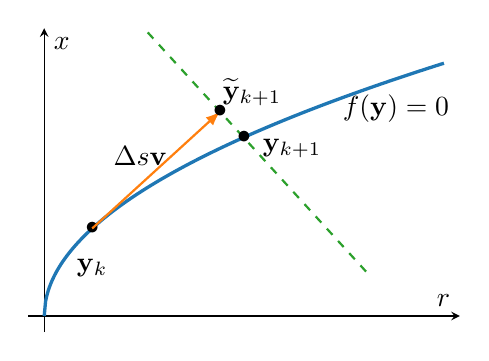
\begin{tikzpicture}[baseline]
        \begin{axis}[
            scale=0.8, % scale
            xmin=-0.1,xmax=2.6,ymin=-0.1,ymax=1.8, % range of plot
            % legend style={at={(axis cs: 1,0)}, anchor=south east}, % position of legends
            unit vector ratio = {1, 1}, % aspect ratio
            axis lines = middle, % middle or box
            %axis x line = bottom, % top, middle, bottom, none: axis x line* = ... removes arrow heads
            %axis y line = left, % left, center, right, none: axis y line* = ... removes arrow heads
            xlabel = {$r$}, ylabel = {$x$}, % axis labels 
            xtick = {-1}, ytick = {-1},
        ]
            \addplot[tab_blue, domain=0.0:2.5, samples=300, very thick] ({x}, {sqrt(x)});   
            \node at (2.2, 1.3) {$f(\mathbf{y})=0$};
            % \addplot[tab_blue, domain=0.0:1.5, samples=100, very thick, dashed] {0};
            % \addplot[tab_blue, domain=0.0:1.5, samples=100, very thick] ({x}, {-sqrt(x)});   
            \node at (0.3, {sqrt{0.3}}) {$\bullet$};
            \node at (0.3, 0.3) {$\mathbf{y}_k$};
            \addplot[tab_orange, domain=0:0.8, -latex, thick] ({0.3+x}, {sqrt{0.3}+x/(2*sqrt(0.3))});
            \node at (1.3, 1.4) {$\widetilde{\mathbf{y}}_{k+1}$}; 
            \addplot[tab_green, domain=-1.0:1.0, thick, dashed] ({0.3+0.8-x/(2*sqrt(0.3))}, {sqrt{0.3}+0.8/(2*sqrt(0.3))+x});
            \node at ({0.3+0.8}, {sqrt{0.3}+0.8/(2*sqrt(0.3))}) {$\bullet$};
            \node at (1.25, 1.115) {$\bullet$};
            \node at (1.55, 1.05) {$\mathbf{y}_{k+1}$};
            \node at (0.6, 1.0) {$\Delta s \mathbf{v}$};
            % \node at (2.2, 3.7) {$r>0$};
            % \node at (2.2, 2.7) {$r<0$};
            % \node[tab_blue] at (1.0, -1/6) {$\bullet$};
            % \addplot3[red, thick, domain=90:300, samples=60, samples y=1]({0.8*sin(x)}, {0.8*cos(x)}, {0});
            % \addplot3[red, variable=\t, samples=7, samples y=1, domain=110:300, -latex, quiver={u={cos(t)}, v={-sin(t)}, scale arrows=0.01}]({0.8*sin(t)}, {0.8*cos(t)}, {0});
        \end{axis}
    \end{tikzpicture}
\end{document}